\chapter{Pruebas y resultados\label{sec:pruebasYResultados}}

En esta sección se presentan las pruebas principales a las que se ha sometido al sistema a lo largo del desarrollo, además de los resultados principales en cada una de ellas. Se divide la sección en dos partes. La primera, se centra en el \textbf{primer prototipo}, correspondiente al \textbf{año académico 2013/2104}, que fue utilizado satisfactoriamente en una asignatura del Grado en Historia. La segunda parte se centra en el \textbf{segundo (y actual) prototipo}, correspondiente al \textbf{año académico 2014/2015}, probado en una asignatura del Grado en Educación Infantil.

% IDEAS A VENDER:
% Generalizable y escalable. Podemos cambiar el modelo subyacente sin sufrir
% Meter el apartado de análisis de resultados
% Se han usado por 50 personas y ha aguantado
% Hablar de la base de datos. Del diseño y cómo se ha hecho
% Probado en entorno real

\section{2013/2014: Primer prototipo}

% Añadir la parte de análsis de datos

Durante el curso académico 2013/2014, 15 alumnos de la asignatura de ``Historia Antigua I'' del Grado en Historia de la Universidad Autónoma de Madrid utilizaron \acrshort{e-valUAM} como \textbf{herramienta de estudio y de evaluación}. Fue el entorno donde se probó el primer prototipo, el cual ya permitía responder cuestionarios, pero no permitía a los profesores crearlos de forma autónoma ni les ofrecía posibilidades multimedia avanzadas (solo se permitía una imagen opcional por pregunta). De esta forma, la experiencia se centró en \textbf{probar la experiencia de uso} de los alumnos, la \textbf{robustez del sistema} para responder a los picos de demanda, además de \textbf{probar los modelos subyacentes}.

\begin{figure}[htp!]
	\centering
	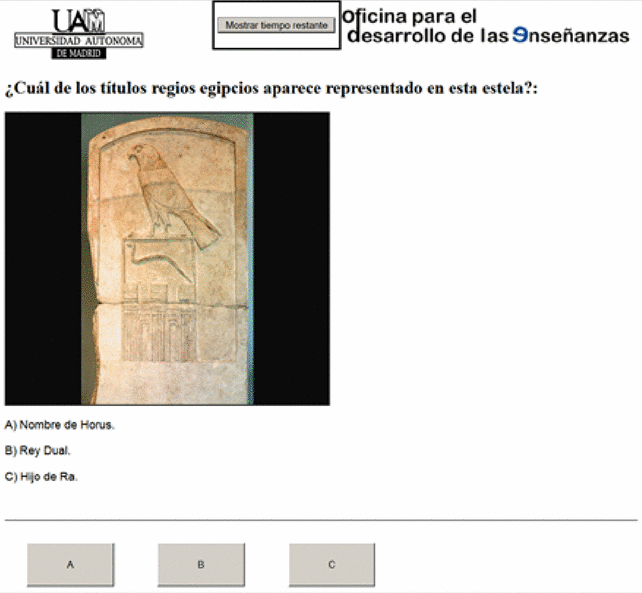
\includegraphics[width=0.75\textwidth,clip=true]{e-valUAM_primera_version}
	\caption{Interfaz del módulo del examen del primer prototipo}
	\label{fig:e-valUAM primera version}
\end{figure}

\begin{table}[hc]
	\centering
	\begin{tabular}{l|l}
		{\bf Cuestionarios}             & 3 de autoevaluación y 4 exámenes \\ 
		{\bf Usuarios}                  & 15 alumnos del Grado en Historia \\
		{\bf Preguntas totales}         & 372                              \\ 
		{\bf Cuestionarios contestados} & 254                              \\ 
		{\bf Preguntas contestadas}     & 12390                            \\ 
		{\bf Ficheros multimedia}		& 178							   \\
	\end{tabular}
	\caption{Datos de uso del primer prototipo.}
	%\label{tab:primer prototipo}
\end{table}

Desde el mes de \textbf{octubre hasta el final del curso}, los alumnos tuvieron disponibles el sistema. Los cuestionarios de autoevaluación eran accesibles tantas veces como quisieran los alumnos, mientras que los de examen solo durante la hora del examen. De los 15 alumnos, 6 utilizaron la aplicación para autoevaluación menos de 3 veces, mientras que otros 6 la utilizaron más de 15 veces. La calificación determinada por la aplicación \textbf{ponderó en la nota final de la asignatura}.

Los resultados de la experiencia fueron muy satisfactorios. A nivel técnico, \textbf{el sistema respondió correctamente}. La mayor prueba de estrés del sistema fue el día del examen final. Los 15 alumnos lo realizaron a la vez, lo que supuso aproximadamente 40 peticiones por minuto al servidor durante los 35 minutos que duró el examen. El sistema logró almacenar todas las respuestas correctamente, seleccionar todas las preguntas siguientes siguiendo el modelo y ningún alumno tuvo que esperar entre preguntas ni sufrió ningún corte del servicio. Tampoco se registró ningún problema en los 3 meses que los alumnos hicieron un uso más intensivo del mismo (de noviembre de 2013 a enero de 2014).

% Hablar de qué se decidió cambiar
Algunos alumnos mostraron malestar con el modelo del examen. Las molestias venían provocadas porque no se pudieran dejar preguntas en blanco ni que se pudiera revisar una respuesta anterior. Aunque la segunda es una imposición del modelo (al depender las nuevas preguntas de las respuestas anteriores, estas no pueden cambiar), la primera sí se tuvo en consideración añadiendo la opción al modelo de la respuesta con duda.

De cara a la creación del \textbf{ segundo prototipo}, además de añadir la respuesta con duda, se decidió crear el \textbf{apartado de gestión del profesor}, además de aumentar las capacidades de la aplicación para trabajar con \textbf{ficheros multimedia}. Así mismo, se hizo una \textbf{actualización de la interfaz} para adaptarla a todas las nuevas posibilidades multimedia que iban a incorporarse.

\section{2014/2015: Segundo prototipo}

Durante el curso académico 2014/2015, \acrshort{e-valUAM} se utilizó en la asignatura de ``El Entorno como Instrumento Educativo'' del Grado en Educación Infantil, de dos formas. Por un lado se utilizó para un \textbf{test sobre el conocimiento informático} de los alumnos que sirvió para obtener información sobre los futuros usuarios y probar un nuevo modelo de adaptación. Por otro lado, se utilizó como \textbf{ parte de la asignatura}.

Las pruebas realizadas en este entorno fueron mucho \textbf{más extensas} que en el curso anterior, por varios motivos. Primero, había \textbf{más alumnos} y por lo tanto la aplicación se enfrentó a mayores picos de demanda. Segundo, se añadió \textbf{más funcionalidad} tanto para los profesores como para los alumnos.

En las siguientes secciones se detallan cómo fueron cada una de las experiencias.
% Contar aquí que cambiamos el modelo

\subsection{Test de conocimientos informáticos}

El objetivo de este test era triple. Buscábamos conocer cuál era el\textbf{ nivel de informática de los alumnos} que después utilizarían el sistema en su asignatura, probar exhaustivamente las \textbf{opción de respuesta con duda} y, por último, crear un \textbf{nuevo modelo de evaluación} utilizando la diferencia entre el conocimiento de expertos (alumnos del Ingeniería Informática) y un grupo de control (alumnos del Educación Infantil).

\begin{table}[hc]
	\centering
	\begin{tabular}{l|p{10cm}}
		{\bf Cuestionarios}             & 1 examen \\ 
		{\bf Usuarios}                  & 83 alumnos: 49 del Grado en Educación Infantil. 34 alumnos del Grado en Ingeniería Informática o el Doble Grado con Matemáticas \\
		{\bf Preguntas totales}         & 60, divididas en dos niveles    \\ 
		{\bf Cuestionarios contestados} & 83                              \\ 
		{\bf Preguntas contestadas}     & 4980                             \\ 
		{\bf Ficheros multimedia}		& 0							   \\
	\end{tabular}
	\caption{Datos de uso del test de conocimientos inform\'aticos.}
\end{table}

Cada pregunta tenía 4 opciones, siendo una de ellas siempre ``No lo sé''. Además, fue el primer examen donde se utilizó la opción de respuesta con duda. Por estas peculiaridades, el modelo descrito en \ref{sec:modelo adapatacion} se varió ligeramente. Todos los alumnos respondían primero a las 30 preguntas del primer nivel y después a las 30 del segundo nivel, sin importar las respuestas previas.

Este cuestionario permitió \textbf{conocer mejor a los futuros usuarios}, además de probar el segundo prototipo del sistema antes de volver a utilizarlo en una asignatura real. Se hizo una prueba de estrés cuando los 25 alumnos de segundo curso de Ing. Informática realizaron a la vez el cuestionario. De nuevo, el sistema no mostró ningún problema. También sirvió para comprobar la \textbf{robustez del diseño} de la aplicación, ya que las modificaciones en el modelo de adaptación solo involucraron realizar cambios menores en uno de los ficheros, lo que parece indicar que la modularización se diseño correctamente.

\subsection{Alumnos del Grado en Educación Infantil}

Los 49 alumnos de ``El Entorno como Instrumento Educativo'' utilizaron \acrshort{e-valUAM} de tres formas distintas:

\begin{enumerate}
 	\item Tuvieron a su disposición un \textbf{cuestionario para la autoevaluación}. 
 	\item Parte de su clasificación final dependió de un \textbf{examen} realizado mediante la plataforma. 
 	\item Como parte de la asignatura tenían que presentar un \textbf{proyecto pedagógico} para niños de educación infantil, que tuvieron que \textbf{plasmar en un cuestionario} de \acrshort{e-valUAM}. 
\end{enumerate}


\begin{table}[hc]
	\centering
	\begin{tabular}{l|l}
		{\bf Cuestionarios}             & 1 autoevaluación y 1 examen \\ 
		{\bf Usuarios}                  & 49 alumnos\\
		{\bf Preguntas totales}         & 244, divididas en cuatro niveles    \\ 
		{\bf Cuestionarios contestados} & 887                              \\ 
		{\bf Preguntas contestadas}     & 6079                             \\ 
		{\bf Ficheros multimedia}		& 21							   \\
	\end{tabular}
	\caption{Datos de uso del segundo prototipo utilizado para evaluaci\'on.}
\end{table}

Desde dicimebre de 2014, los alumnos tuvieron accesible el cuestionario de autoevaluación. El 14 de enero de 2015, realizaron el examen final utilizando también \acrshort{e-valUAM}. Los 50 alumnos acudieron a los laboratorios de la EPS para realizar el examen de 40 preguntas durante 60 minutos. Se utilizaron parte de preguntas de autoevaluación, algunas sin alterar, otras modificando los datos. También se añadieron preguntas nuevas.

Este examen sirvió como nueva prueba de estrés del sistema. Durante 40 minutos, 49 alumnos accedieron en simultáneo, realizando de media unas 75 peticiones por minuto al servidor. Como en todas las ocasiones anteriores, no hubo ningún problema con la aplicación y toda la información quedó correctamente guardada.

Después del examen, se dio una charla de 15 minutos a los alumnos para explicarles cómo debían utilizar la interfaz del profesor, la cual tuvieron que utilizar para entregar un trabajo que se les exigía en la asignatura.

\begin{table}[hc]
	\centering
	\begin{tabular}{l|l}
		{\bf Cuestionarios}             & 19 \\ 
		{\bf Usuarios}                  & 49 alumnos, actuando como docentes\\
		{\bf Preguntas totales}         & 848  \\ 
		{\bf Cuestionarios contestados} & 0                              \\ 
		{\bf Preguntas contestadas}     & 0                             \\ 
		{\bf Ficheros multimedia}		& 1364							   \\
	\end{tabular}
	\caption{Datos de uso del segundo prototipo utilizado para la entrega del trabajo.}
	%\label{tab:test informatica}
\end{table}

Para resolver incidencias o dudas, se puso a disposición de los alumnos un correo electrónico de contacto. Escribieron en total 4 personas, con 2 incidencias y 1 petición de nueva funcionalidad. Finalmente, el profesor de la asignatura corrigió el trabajo accediendo a la sección de profesor y consultando directamente los cuestionarios que cada grupo de alumnos había confeccionado.

\section{Comparativa con otras soluciones}

Para comparar el sistema propuesto, de todas las herramientas disponibles, \textbf{se ha elegido SIETTE} (siglas de \textit{Sistema de Evaluación Inteligente mediante Tests para la Tele educación}), un sistema desarrollado principalmente por Ricardo Conejo Muñoz y Eduardo Guzmán De los Riscos, ambos del grupo $(IA)^2$, de la Universidad de Málaga. Se ha elegido SIETTE al ser un sistema con unos \textbf{objetivos muy similares} al nuestro con una \textbf{larga historia, completamente asentado y probado}. Se encuentra disponible en  \url{http://www.siette.org/siette/}

SIETTE se empezó a desarrollar en los 90 como el \textbf{componente de generación de exámenes adaptativos} de un sistema mayor cuyo objetivo era la clasificación e identifiación de distintas especies vegetales europeas, además de promover el conocimiento sobre ellas. El proyecto, conocido como TREE, se componía del sistema de generación de exámenes (SIETTE), un \textit{Intelligent Tutoring System} y un sistema experto encargado de la clasificación de las especies vegetales\cite{Rios98}. Desde entonces SIETTE ha evolucionado siendo utilizada en \textbf{nuevos dominios}, como la educación infantil\cite{Trella08} o evaluación colaborativa \cite{Conejo09}.

Tanto SIETTE como e-valUAM se engloban dentro de los \acrshort{CAT}, aunque SIETTE se centra en técnicas de la \textit{Item Response Theory} (\acrshort{IRT}) y de la \textit{Classical Test Theory} (\acrshort{CTT}) mientras que e-valUAM se fija más en la \acrshort{AEH}.

Aún así, SIETTE y e-valUAM presentan muchas \textbf{similitudes}. La abstracción que SIETTE realiza del dominio de la evaluación es bastante similar al explorado en e-valUAM, como se puede ver en la figura \ref{fig:SIETTE workflow}, en la que se presenta el flujo de trabajo de SIETTE. 

\begin{figure}[htp!]
	\centering
	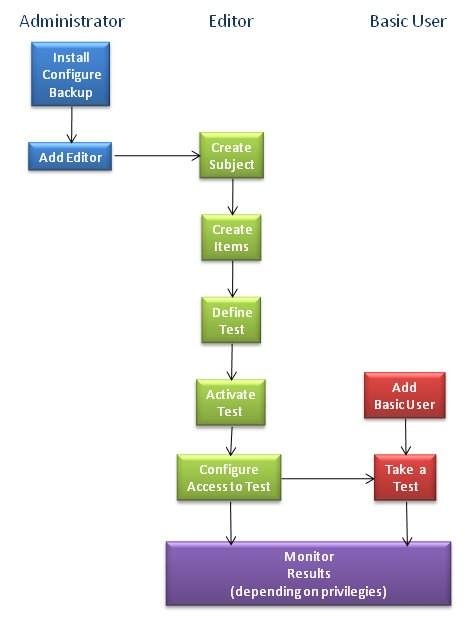
\includegraphics[width=1\textwidth,clip=true]{WorkflowSIETTE}
	\caption{Flujo de trabajo propuesto por SIETTE\cite{SIETTEWiki}}
	\label{fig:SIETTE workflow}
\end{figure}

Lo que en SIETTE son editors, subjects, items y tests, en e-valUAM son profesores, materias, preguntas y cuestionarios y el flujo de trabajo es prácticamente idéntico. En un pricipio SIETTE permitía que una pregunta perteneciera a uno o varios temas, y que los exámenes estuvieran compuestos de uno o varios temas, pudiendo estar un tema en varios exámenes\cite{Conejo04}. Sin embargo, las últimas versiones de SIETTE siguen una estructura jerárquica en la que cada pregunta corresponde a un tema, \textbf{idéntico al modelo de e-valUAM}. Así mismo, tanto SIETTE como e-valUAM poseen módulos de análisis de resultados. 

SIETTE, sin embargo, también plantea importantes \textbf{diferencias} con e-valUAM. En general, podemos decir que SIETTE es un sistema \textbf{más maduro y completo} que e-valUAM. Mientras que en e-valUAM solo se permiten crear preguntas de opción múltiple y respuesta simpel, en SIETTE se implementan \textbf{varios tipos de preguntas} adicionales:

\begin{itemize}
	\item Opción múltiple y respuestas múltiple.
	\item Respuesta corta y abierta, en la que se define un patrón que caracteriza a todas las respuestas correctas.
	\item Preguntas generativas, en las que un código genera cada vez una pregunta distinta.
\end{itemize}

El \textbf{análisis de resultados} también es más extenso. SIETTE presenta una característica que permite a los profesores definir errores conceptuales que pueden tener los alumnos en una materia y definir unas reglas que caractericen las respuestas que comentan dichos errores. Una vez definida esta información, el sistema genera informes indicando qué alumnos han cometido qué errores conceptuales.

Otra diferencia importante es que aunque en e-valUAM se han probado varios sistemas de adaptación distintos que han derivado en varias formas de clasificar distintos, aún no se le permite al profesor elegir qué sistema desea aplicar desde su interfaz de configuración. SIETTE tiene desarrollados tres \textbf{métodos de evaluación distintos} (por puntos, porcentual o por \acrshort{IRT}) que están disponibles para los docentes.

